\begin{enumerate}[label=\thechapter.\arabic*,ref=\thechapter.\theenumi]
\item Consider a continuous-time signal $x\brak{t}$ \,defined by $x\brak{t}=0$\,for $\abs{t}>1$, and $x\brak{t}=1-\abs{t}$ for $\abs{t}\le 1$. Let the Fourier transform of $x\brak{t}$ be defined as $X\brak{\omega}=\int_{-\infty}^{\infty}x\brak{t}e^{-j\omega t} dt$. The maximum magnitude of $X\brak{\omega}$ is $\hbox to 4em{\thinspace\hrulefill\thinspace}$.
\hfill{(GATE 2021 EE 43)}
\solution
\iffalse
\let\negmedspace\undefined
\let\negthickspace\undefined
\documentclass[journal,12pt,onecolumn]{IEEEtran}
\usepackage{cite}
\usepackage{amsmath,amssymb,amsfonts,amsthm}
\usepackage{algorithmic}
\usepackage{graphicx}
\usepackage{textcomp}
\usepackage{xcolor}
\usepackage{txfonts}
\usepackage{listings}
\usepackage{enumitem}
\usepackage{mathtools}
\usepackage{gensymb}
\usepackage{comment}
\usepackage{caption}
\usepackage[breaklinks=true]{hyperref}
\usepackage{tkz-euclide} 
\usepackage{listings}
\usepackage{gvv}                                        
\def\inputGnumericTable{}                                 
\usepackage[latin1]{inputenc}                                
\usepackage{color}                                            
\usepackage{array}                                            
\usepackage{longtable}                                       
\usepackage{calc}                                             
\usepackage{multirow}                                         
\usepackage{hhline}                                           
\usepackage{ifthen}                                           
\usepackage{lscape}

\newtheorem{theorem}{Theorem}[section]
\newtheorem{problem}{Problem}
\newtheorem{proposition}{Proposition}[section]
\newtheorem{lemma}{Lemma}[section]
\newtheorem{corollary}[theorem]{Corollary}
\newtheorem{example}{Example}[section]
\newtheorem{definition}[problem]{Definition}
\newcommand{\BEQA}{\begin{eqnarray}}
\newcommand{\EEQA}{\end{eqnarray}}
\newcommand{\define}{\stackrel{\triangle}{=}}
\theoremstyle{remark}
\newtheorem{rem}{Remark}
\begin{document}

\bibliographystyle{IEEEtran}
\vspace{3cm}

\title{GATE 2021 EE 43}
\author{EE23BTECH11022 - G DILIP REDDY}
\maketitle

\bigskip

\renewcommand{\thefigure}{\arabic{figure}}
\renewcommand{\thetable}{\arabic{table}}
\textbf{Question}:\\
Consider a continuous-time signal $x\brak{t}$ \,defined by $x\brak{t}=0$\,for $\abs{t}>1$, and $x\brak{t}=1-\abs{t}$ for $\abs{t}\le 1$. Let the Fourier transform of $x\brak{t}$ be defined as $X\brak{\omega}=\int_{-\infty}^{\infty}x\brak{t}e^{-j\omega t} dt$. The maximum magnitude of $X\brak{\omega}$ is $\hbox to 4em{\thinspace\hrulefill\thinspace}$.
\hfill{(GATE 2021 EE 43)}
\\\\
\solution
\fi
\begin{align}
X\brak{f}&=\int_{-\infty}^{\infty}x\brak{t}e^{-j2\pi f t} dt\\
X\brak{f}&=\int_{-1}^{1}\brak{1-\abs{t}}e^{-j2\pi f t} dt\\
X\brak{f}&=\int_{-1}^{1}e^{-j2\pi f t} 
dt - \int_{-1}^{1}\abs{t}e^{-j2\pi f t} dt\\
X\brak{f}&=2\int_{0}^{1}\cos\brak{{2\pi f t}}
dt - 2\int_{0}^{1}t\cos\brak{2\pi f t} dt\\
X\brak{f}&=2\frac{\sin\brak{{2\pi f }}}{2\pi f}
- 2\sbrak{\frac{\sin\brak{2\pi f }}{2\pi f}+\frac{\cos\brak{2\pi f }}{\brak{2\pi f}^2}-\frac{1}{\brak{2\pi f }^2}}\\
X\brak{f}&=2\frac{1-\cos\brak{2\pi f }}{\brak{2\pi f}^2}\\
X\brak{f}&=2\frac{2\sin^2\brak{\frac{2\pi f}{2}}}{\brak{2\pi f}^2}\\
X\brak{f}&=\frac{\sin^2\brak{\pi f}}{\brak{\pi f}^2}\\
f& \to 0 \implies X\brak{f}\to1
\end{align}
Maximum of magnitude of $X\brak{f}=1$
\begin{figure}[h]
    \centering
    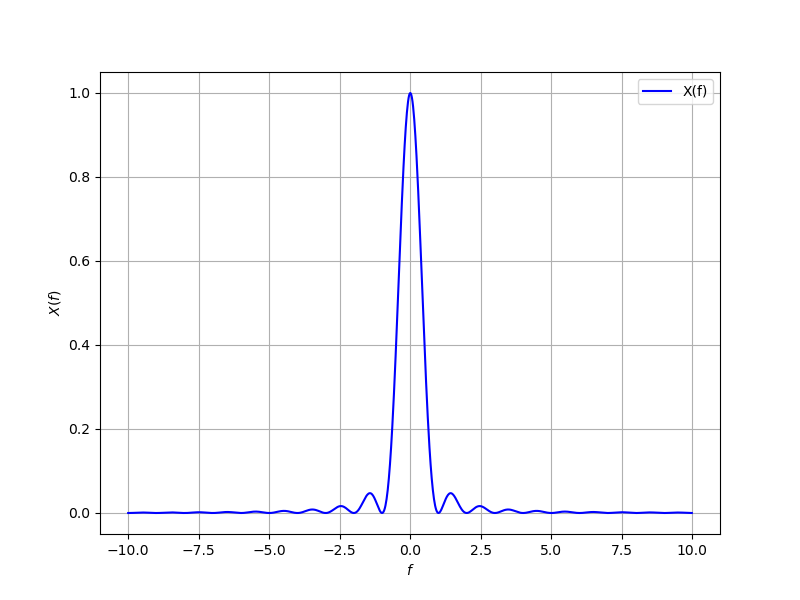
\includegraphics[width=1\linewidth]{2021/EE/43/figs/graph.png}
    \caption{plot of X(f)}
\end{figure}
%\end{document}

\pagebreak
\end{enumerate}
